% Options for packages loaded elsewhere
\PassOptionsToPackage{unicode}{hyperref}
\PassOptionsToPackage{hyphens}{url}
%
\documentclass[
]{article}
\usepackage{amsmath,amssymb}
\usepackage{iftex}
\ifPDFTeX
  \usepackage[T1]{fontenc}
  \usepackage[utf8]{inputenc}
  \usepackage{textcomp} % provide euro and other symbols
\else % if luatex or xetex
  \usepackage{unicode-math} % this also loads fontspec
  \defaultfontfeatures{Scale=MatchLowercase}
  \defaultfontfeatures[\rmfamily]{Ligatures=TeX,Scale=1}
\fi
\usepackage{lmodern}
\ifPDFTeX\else
  % xetex/luatex font selection
\fi
% Use upquote if available, for straight quotes in verbatim environments
\IfFileExists{upquote.sty}{\usepackage{upquote}}{}
\IfFileExists{microtype.sty}{% use microtype if available
  \usepackage[]{microtype}
  \UseMicrotypeSet[protrusion]{basicmath} % disable protrusion for tt fonts
}{}
\makeatletter
\@ifundefined{KOMAClassName}{% if non-KOMA class
  \IfFileExists{parskip.sty}{%
    \usepackage{parskip}
  }{% else
    \setlength{\parindent}{0pt}
    \setlength{\parskip}{6pt plus 2pt minus 1pt}}
}{% if KOMA class
  \KOMAoptions{parskip=half}}
\makeatother
\usepackage{xcolor}
\usepackage{graphicx}
\makeatletter
\def\maxwidth{\ifdim\Gin@nat@width>\linewidth\linewidth\else\Gin@nat@width\fi}
\def\maxheight{\ifdim\Gin@nat@height>\textheight\textheight\else\Gin@nat@height\fi}
\makeatother
% Scale images if necessary, so that they will not overflow the page
% margins by default, and it is still possible to overwrite the defaults
% using explicit options in \includegraphics[width, height, ...]{}
\setkeys{Gin}{width=\maxwidth,height=\maxheight,keepaspectratio}
% Set default figure placement to htbp
\makeatletter
\def\fps@figure{htbp}
\makeatother
\ifLuaTeX
  \usepackage{luacolor}
  \usepackage[soul]{lua-ul}
\else
  \usepackage{soul}
\fi
\setlength{\emergencystretch}{3em} % prevent overfull lines
\providecommand{\tightlist}{%
  \setlength{\itemsep}{0pt}\setlength{\parskip}{0pt}}
\setcounter{secnumdepth}{-\maxdimen} % remove section numbering
\ifLuaTeX
  \usepackage{selnolig}  % disable illegal ligatures
\fi
\usepackage{bookmark}
\IfFileExists{xurl.sty}{\usepackage{xurl}}{} % add URL line breaks if available
\urlstyle{same}
\hypersetup{
  pdftitle={Applied Multi-Agent Learning and Imperfect Information Games},
  hidelinks,
  pdfcreator={LaTeX via pandoc}}

\title{Applied Multi-Agent Learning and Imperfect Information Games}
\author{}
\date{}

\begin{document}
\maketitle

\textbf{Applied Multi-Agent Learning \& Imperfect Information Games:
Lessons from Libratus and Pluribus (and their foundations)}

Mauricio Garcia

University of Texas - Austin

February 2025

\textbf{\ul{ABSTRACT}}

This paper traces the evolution of game-solving AI from
perfect-information milestones (DeepBlue, AlphaGo) to the cutting edge
of imperfect-information and multi-agent learning (Libratus, Pluribus).
We review the core concepts: Nash equilibrium, minimax, and
Counterfactual Regret Minimization, then show how abstraction, blueprint
strategies, and real-time subgame solving enable superhuman performance
in two- and multi-player no-limit Texas Hold'em poker. Finally, we
distill key lessons about tractability versus exploitability, the
necessity of live adaptation against human opponents, and the future
role of richer opponent modeling and interactive interfaces.

\textbf{\ul{INTRODUCTION}}

In the realm of artificial intelligence, games have long served as
benchmarks for measuring progress and testing new algorithms.

In 1997, IBM\textquotesingle s DeepBlue made history by defeating world
chess champion Garry Kasparov, marking a significant milestone in
perfect-information games. However, the challenge of
imperfect-information games, where players must make decisions with
hidden information, remained a formidable frontier.

In January 2017, 20 years later, Carnegie Mellon
University\textquotesingle s Libratus became the first AI to defeat
professional players in heads-up no-limit Texas Hold\textquotesingle em
poker, a benchmark for imperfect-information game solving.

This achievement was followed by another breakthrough in July 2019, when
Carnegie Mellon University and Meta AI researchers developed Pluribus,
an AI capable of winning in multiplayer poker games against professional
players.

These advancements not only demonstrate the potential of AI in complex
computational game-solving environments but also highlight the evolving
capabilities of AI systems: DeepBlue\textquotesingle s strategic depth
in perfect-information games, Libratus\textquotesingle s mastery of
two-player imperfect-information scenarios, and
Pluribus\textquotesingle s ability to navigate the intricate dynamics of
multiplayer interactions, showcasing the progress in multi-agent
learning.

\textbf{\ul{HISTORICAL CONTEXT - DEEPER DIVE}}

\textbf{\ul{ADVANCEMENTS IN GAME SOLVING MODELS}}

The evolution of artificial intelligence in game-solving has been marked
by a series of groundbreaking achievements, each pushing the boundaries
of what machines can accomplish in strategic environments.

\begin{enumerate}
\def\labelenumi{\arabic{enumi}.}
\item
  \textbf{\ul{DeepBlue: A Milestone in Perfect-Information Games}}
\end{enumerate}

\begin{quote}
This journey began with \emph{\ul{IBM\textquotesingle s DeepBlue}},
which, in 1997, became the first computer system to defeat a reigning
world chess champion, Garry Kasparov. Chess, a perfect-information game,
provided a structured environment where both players had complete
visibility of the game state. DeepBlue\textquotesingle s success was
largely attributed to its brute-force search capabilities, evaluating
millions of positions per second, combined with sophisticated heuristics
to prune the search space effectively.
\end{quote}

\begin{enumerate}
\def\labelenumi{\arabic{enumi}.}
\setcounter{enumi}{1}
\item
  \textbf{\ul{AlphaGo: Advancing AI with Deep Learning}}
\end{enumerate}

\begin{quote}
Following DeepBlue, another significant milestone came with
\emph{\ul{Google\textquotesingle s AlphaGo}}, which achieved a historic
victory over 18-time world champion Go player,
\href{https://en.wikipedia.org/wiki/Lee_Sedol}{\ul{Lee Sedol}}, in 2016.
Go, unlike chess, presents a vastly larger search space and requires a
more nuanced understanding of strategy and intuition.
AlphaGo\textquotesingle s success was driven by the integration of deep
neural networks and the Monte Carlo tree search, allowing it to evaluate
positions and potential moves with unprecedented accuracy. This
combination enabled AlphaGo to learn and improve its strategies through
self-play, marking a shift from brute-force computation to more
sophisticated learning techniques.
\end{quote}

\begin{enumerate}
\def\labelenumi{\arabic{enumi}.}
\setcounter{enumi}{2}
\item
  \textbf{\ul{Transition to Imperfect-Information Games\ldots{}}}
\end{enumerate}

\begin{quote}
These advancements in perfect-information games laid the groundwork for
tackling more complex games characterized by hidden information. Unlike
chess and Go, where all information is visible to both players,
imperfect-information games like poker involve uncertainty and require
players to make decisions based on incomplete information. This
introduces additional layers of complexity, as players must account for
hidden variables and potential deception by opponents.
\end{quote}

\begin{enumerate}
\def\labelenumi{\arabic{enumi}.}
\setcounter{enumi}{3}
\item
  \textbf{\ul{Libratus and Pluribus: Mastering Imperfect-Information
  Games}}
\end{enumerate}

\begin{quote}
Libratus and Pluribus exemplify this progress.
Libratus\textquotesingle s victory in Texas Hold\textquotesingle em
poker demonstrated that AI could achieve superhuman performance in
two-player imperfect-information games. Pluribus extended this success
to multiplayer settings, showcasing the potential of AI to handle even
more complex interactions involving multiple agents.
\end{quote}

\textbf{\ul{IMPERFECT INFORMATION GAMES}}

Look into older imperfect information games, older, and can write
history about this (milestones). This visualization I found can guide
this text.

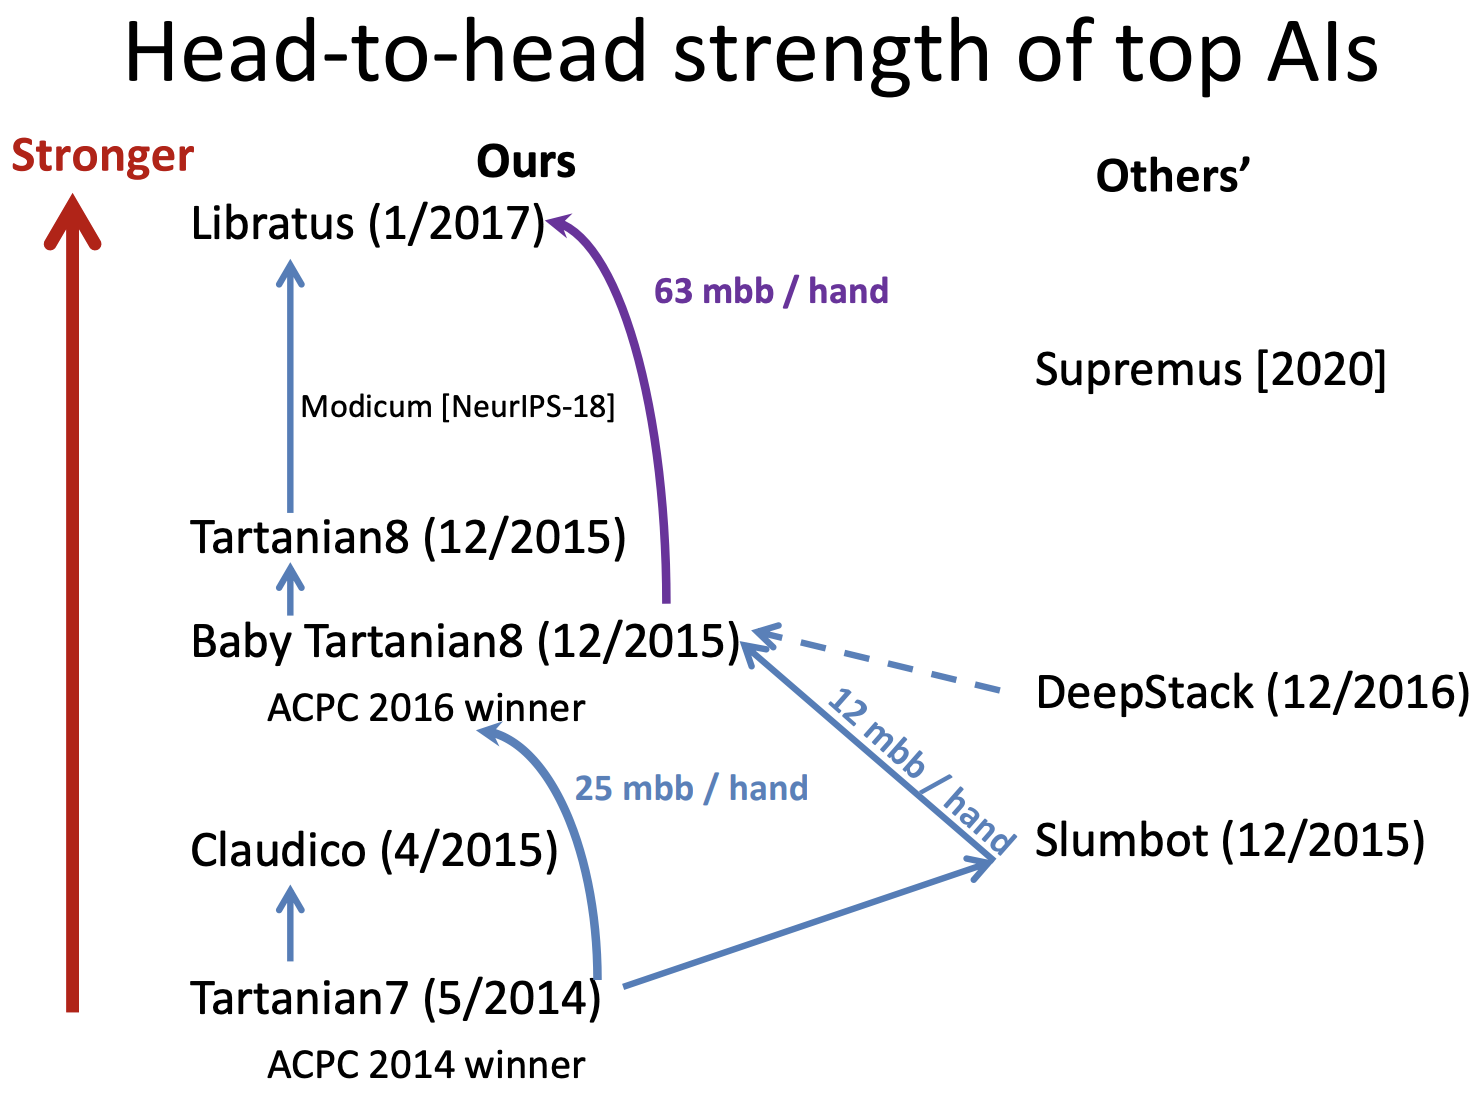
\includegraphics[width=6.26772in,height=4.66667in]{media/media/image4.png}

\textbf{\ul{MULTI-AGENT LEARNING}}

Look into older/other multi-agent learning examples \& research areas,
can write history about this (milestones)

\textbf{\ul{BROADER IMPLICATIONS}}

These models have not only advanced the field of AI but have also paved
the way for applications in real-world scenarios where decision-making
under uncertainty is crucial. From negotiations and cybersecurity to
financial markets and strategic planning, the techniques developed for
game solving are increasingly being adapted to address challenges in
diverse domains.

\textbf{\ul{ABOUT TEXAS HOLD\textquotesingle EM POKER}}

Texas Hold\textquotesingle em is one of the most popular and
strategically complex variants of poker, making it an ideal testing
ground for artificial intelligence research in imperfect-information
games. The game is played with a standard 52-card deck and involves
multiple players, each with private "hole cards" and shared community
cards. Additionally, "poker" refers to the general card game played with
multiple players at a table, while "heads up poker" specifically means a
poker game played between only two players.

\textbf{\ul{WHY IT IS A USEFUL IMPERFECT INFORMATION GAME:}}

\begin{enumerate}
\def\labelenumi{\arabic{enumi}.}
\item
  Each player\textquotesingle s hole cards are private. This creates
  uncertainty about the opponents' hands. Players must infer the
  possible holdings of others based on their actions and betting
  patterns.
\item
  Deceptive or Strategic Maneuvers: Bluffing, semi-bluffing, and
  slow-playing (a player plays a strong hand weakly to encourage
  opponents to stay in the pot) are all techniques that can be played.
  Players must balance aggression with caution.
\item
  The dynamics throughout the game change. For example, the community
  cards can completely change the strength of a player's hand.
\item
  The decision-making processes in poker mirror those in many real-world
  scenarios, such as negotiations, financial markets, competitive
  business environments, etc.. To elaborate, players must weigh risks
  and rewards, anticipate the actions of others, and make decisions with
  incomplete information.
\end{enumerate}

Rules:

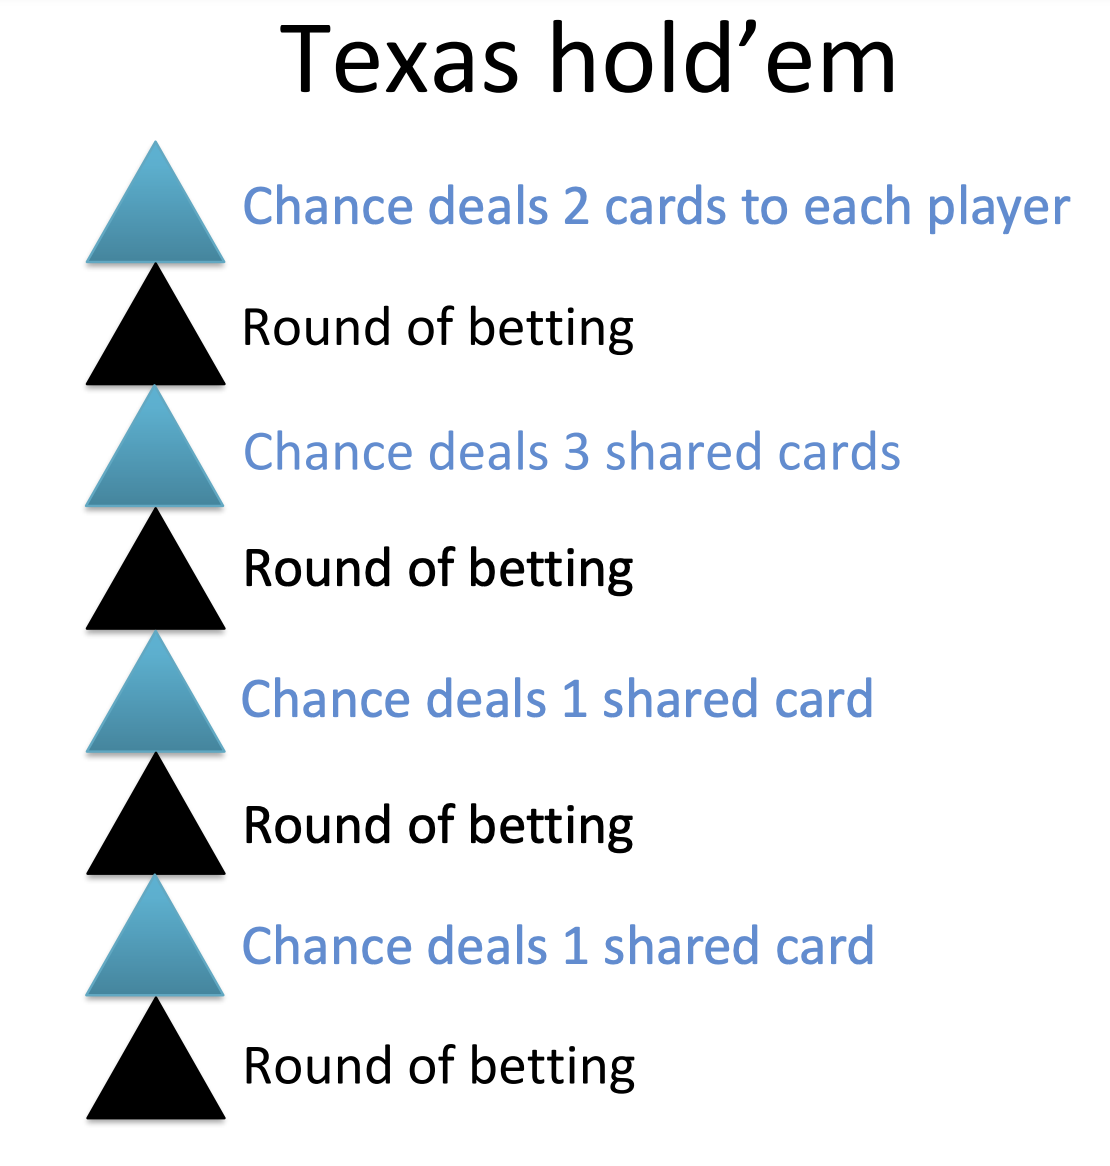
\includegraphics[width=3.76382in,height=3.95139in]{media/media/image1.png}

\textbf{\ul{KEY FOUNDATIONAL CONCEPTS USED TO BUILD LIBRATUS \&
PLURIBUS:}}

\textbf{\ul{EQUILBRIUM CONCEPTS:}}

\textbf{\ul{NASH EQUILIBRIUM:}}

\begin{quote}
\textbf{\ul{Definition:}}

Nash equilibrium is a game theory concept that describes when no player
can improve their outcome by changing their strategy. It represents a
stable state where each player\textquotesingle s strategy is optimal
given the strategies of all other players.

\textbf{\ul{Application in AI:}}

In the context of poker, Nash equilibrium provides a framework for
developing strategies that are robust against exploitation.
\end{quote}

\textbf{\ul{VON NEUMANN'S MINIMAX THEOREM:}}

\begin{quote}
\textbf{\ul{Definition:}}

Originally developed by John von Neumann before WW2, the minimax theorem
is a foundational pillar of game theory. It states that in zero-sum
games, there exists a strategy for each player that minimizes their
maximum possible loss, effectively balancing offensive and defensive
considerations.
\end{quote}

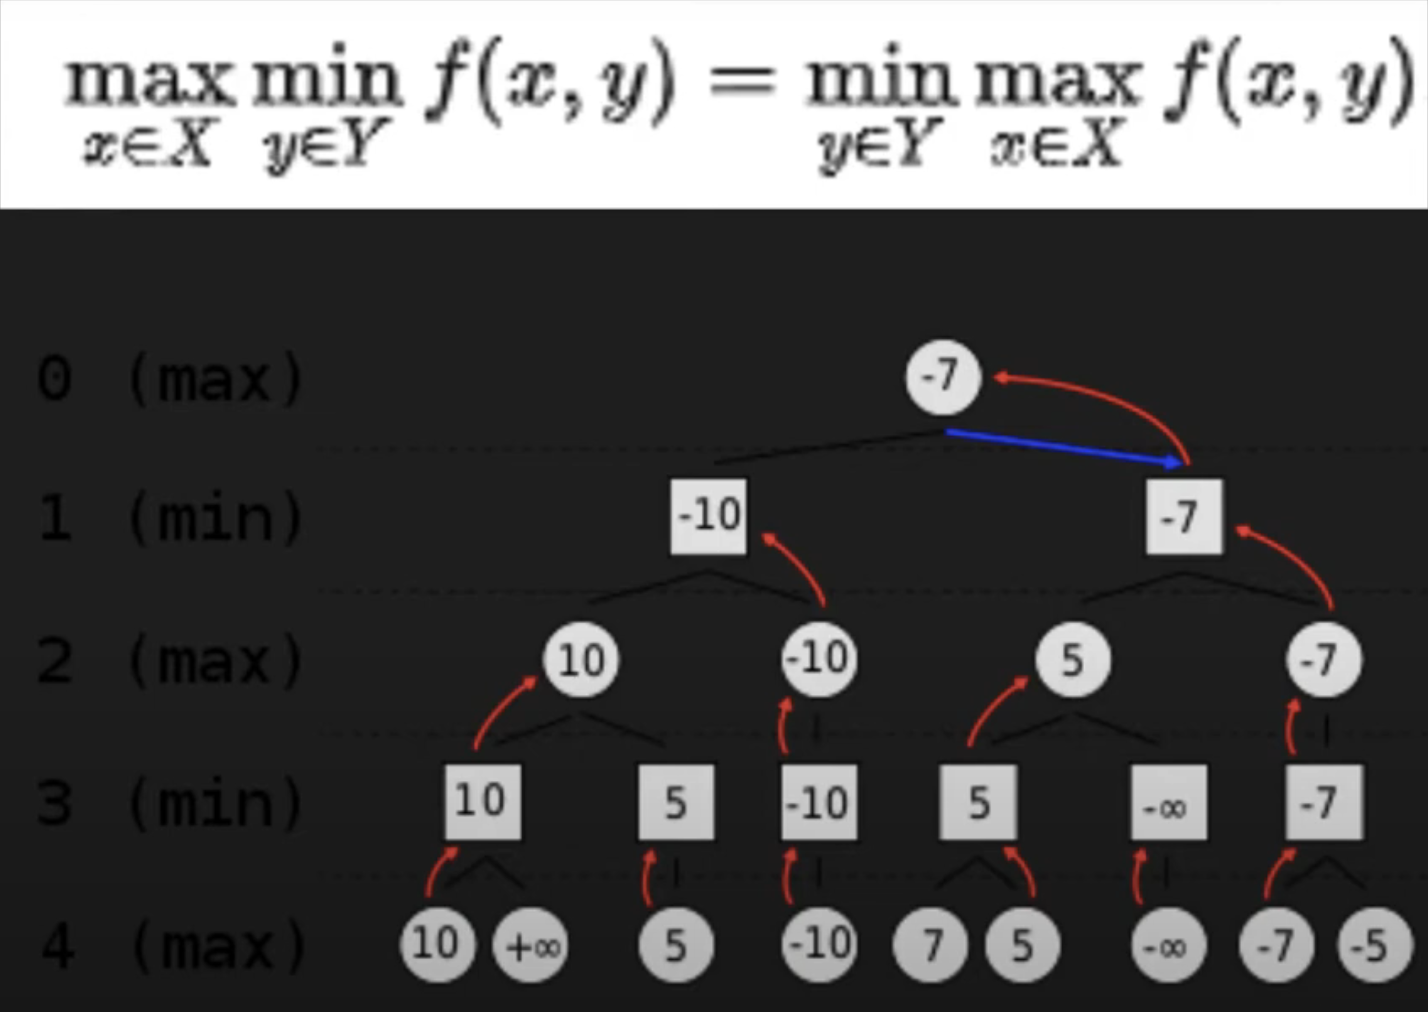
\includegraphics[width=6.26772in,height=4.44444in]{media/media/image6.png}

\begin{quote}
\textbf{\ul{Why it is relevant, although not explicitly mentioned in the
main research papers:}}

While the minimax theorem is not explicitly mentioned in the research
papers, its principles are relevant to heads-up poker, which is treated
as a zero-sum game. Libratus leverages these principles to develop
strategies that minimize potential losses while maximizing gains.

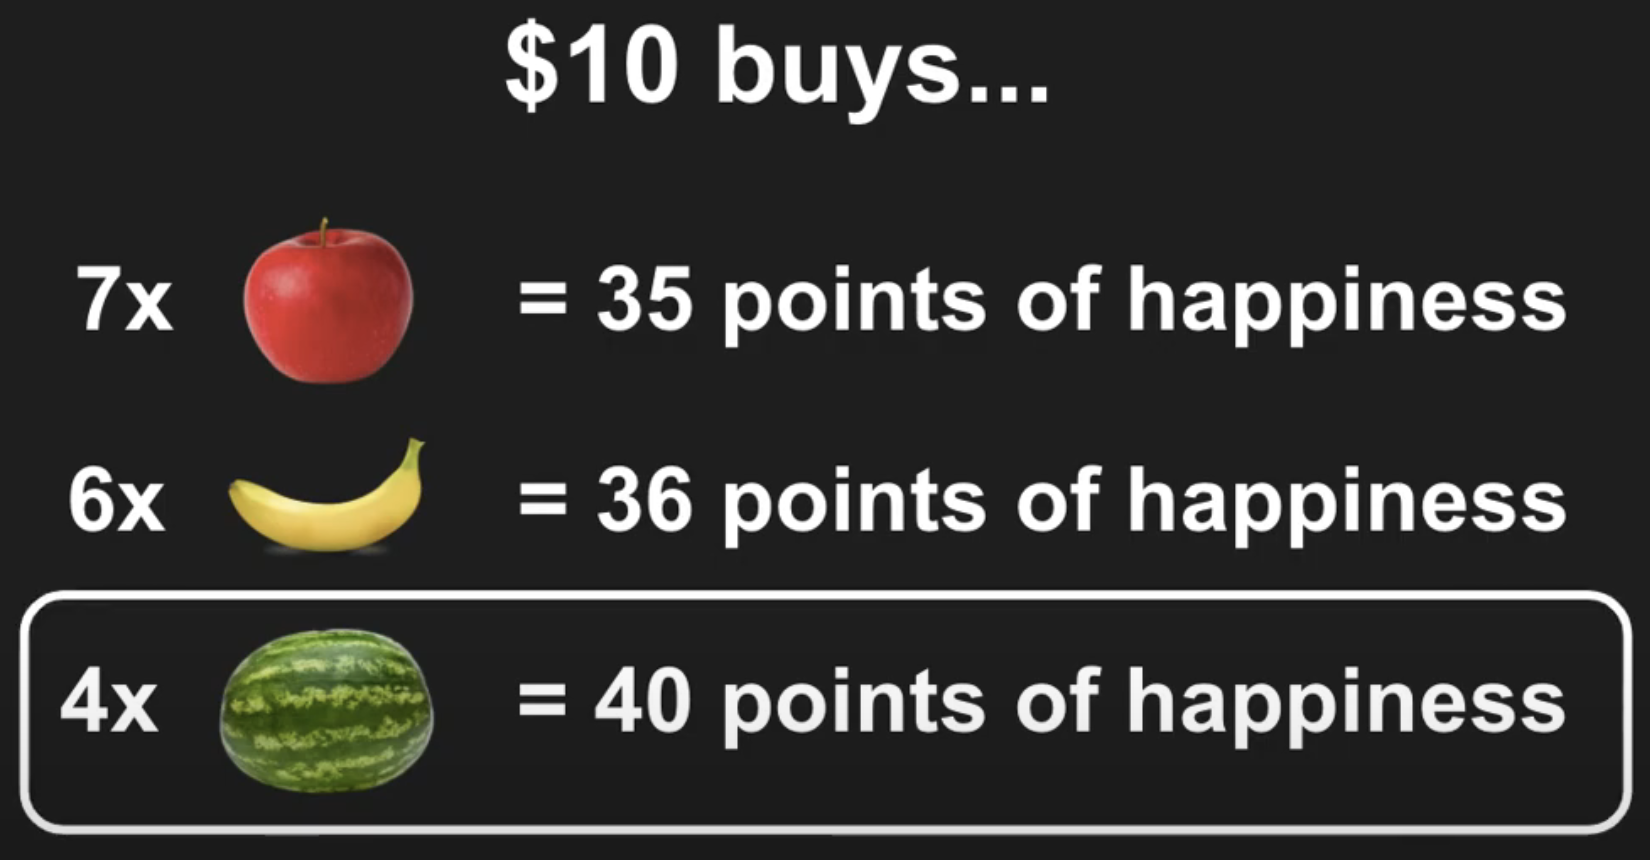
\includegraphics[width=6.26772in,height=3.26389in]{media/media/image3.png}

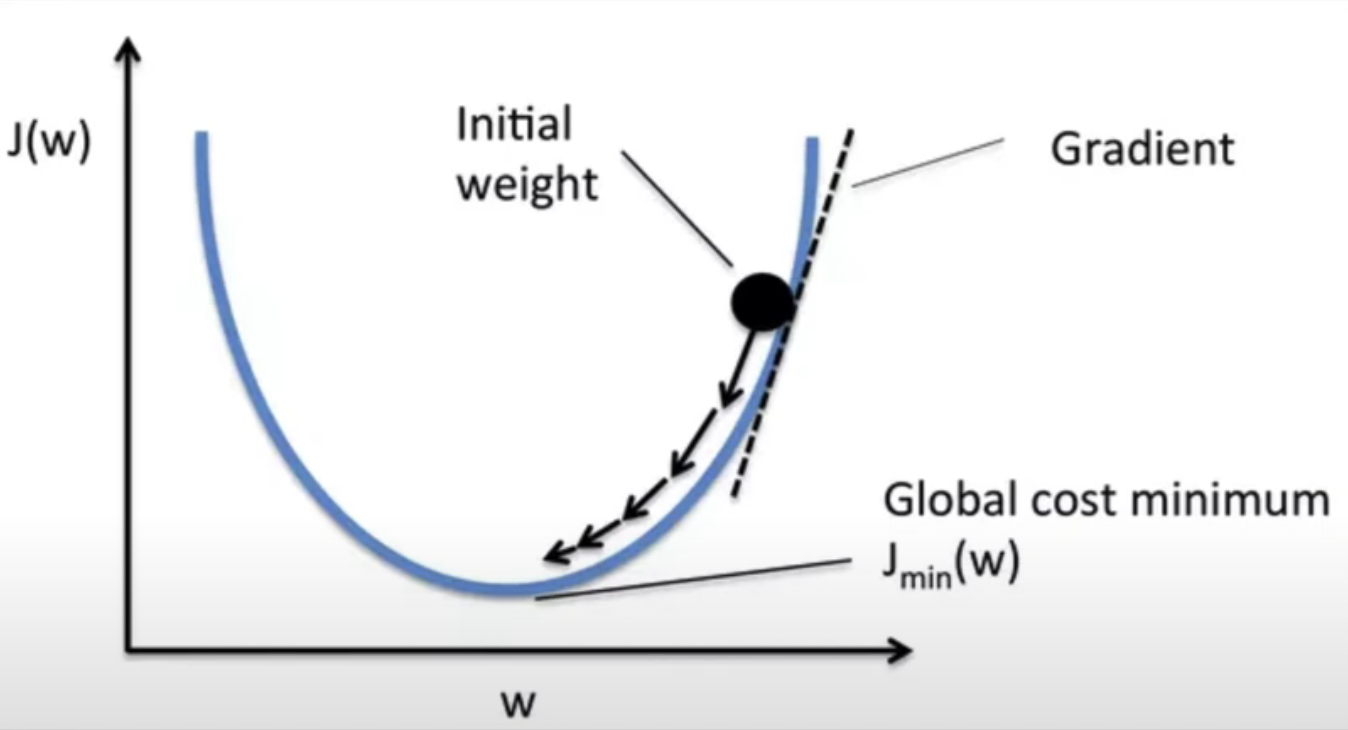
\includegraphics[width=6.26772in,height=3.38889in]{media/media/image2.png}
\end{quote}

\textbf{\ul{COUNTERFACTUAL REGRET MINIMIZATION (CFR):}}

CFR is particularly suited for games where players don\textquotesingle t
have complete information about the state of the game, like in poker,
where players only see their own cards. The core concept is to minimize
the "regret" a player feels for not choosing a different action at each
decision point, considering the possible outcomes based on the
counterfactual scenario.

\begin{quote}
\textbf{\ul{HOW IT WORKS:}}

CFR works by repeatedly traversing the game tree, calculating regrets
for each action at each decision point, and adjusting the
player\textquotesingle s strategy based on these regrets. A
\href{http://modelai.gettysburg.edu/2013/cfr/cfr.pdf}{\ul{key element of
CFR is calculating the "reach probability" of each decision point}},
which represents the likelihood of reaching that point in the game based
on the current strategies.

\textbf{\ul{Step by step:}}
\end{quote}

\begin{enumerate}
\def\labelenumi{\arabic{enumi}.}
\item
  Initialize:

  \begin{enumerate}
  \def\labelenumii{\alph{enumii}.}
  \item
    Start with a uniform random strategy for each player at every
    decision point.
  \end{enumerate}
\item
  Traverse the game tree:

  \begin{enumerate}
  \def\labelenumii{\alph{enumii}.}
  \item
    For each iteration, traverse the game tree from the root node,
    calculating the reach probability at each decision point.
  \end{enumerate}
\item
  Calculate regrets:

  \begin{enumerate}
  \def\labelenumii{\alph{enumii}.}
  \item
    At each decision point, calculate the "regret" for each action,
    which represents the difference in expected utility if that action
    had been chosen instead of the one that was chosen.
  \end{enumerate}
\item
  Update strategy:

  \begin{enumerate}
  \def\labelenumii{\alph{enumii}.}
  \item
    Based on the calculated regrets, adjust the player\textquotesingle s
    strategy at each decision point using a "regret-matching" mechanism,
    giving higher probabilities to actions with higher regrets.
  \end{enumerate}
\item
  Repeat:

  \begin{enumerate}
  \def\labelenumii{\alph{enumii}.}
  \item
    Continue iterating through the game tree, updating strategies based
    on calculated regrets until convergence is reached (regrets become
    negligible).
  \end{enumerate}
\end{enumerate}

\textbf{\ul{LIBRATUS:}}

\textbf{\ul{SUMMARY:}}

\begin{quote}
Libratus is an AI system developed by Noam Brown and Tuomas Sandholm at
Carnegie Mellon University, designed to play heads-up (two-player)
no-limit Texas Hold\textquotesingle em poker. In a 20-day, 120,000-hand
competition, Libratus defeated four top human specialist professionals,
marking a significant milestone in AI\textquotesingle s ability to
handle imperfect-information games (Brown \& Sandholm, 2018). This
achievement demonstrated that AI could achieve superhuman performance in
strategic environments characterized by hidden information and
uncertainty.
\end{quote}

\textbf{\ul{HOW IT WORKS (HIGH LEVEL):}}

\begin{itemize}
\item
  Libratus uses application-independent techniques to compute a
  blueprint for the overall strategy, flesh out details for subgames
  reached during play, and improve upon potential weaknesses identified
  by opponents (Brown \& Sandholm, 2018).
\item
  Abstraction (and Blueprint Strategy):

  \begin{itemize}
  \item
    The first module of Libratus computes an abstraction of the game,
    simplifying it while retaining strategic aspects (for example, \$100
    is not so different to \$101). This process reduces the complexity
    of the game while preserving its essential strategic elements.
  \item
    The abstraction allows Libratus to develop a comprehensive strategy
    for the early stages of the game, known as the "blueprint strategy."
    For the later stages, this blueprint provides a general framework
    that can be refined as the game progresses.
  \end{itemize}
\item
  Nested Subgame Solving:

  \begin{itemize}
  \item
    When a later part of the game is reached, Libratus constructs a
    finer-grained abstraction for that subgame and solves it in real
    time. This nested subgame solving ensures that the solution fits
    within the larger blueprint strategy, providing a provable safety
    guarantee.
  \end{itemize}
\item
  Self-Improving Algorithm:

  \begin{itemize}
  \item
    Libratus enhances the blueprint strategy by filling in missing
    branches and computing game-theoretic strategies for those branches.
    This self-improvement is guided by the opponents\textquotesingle{}
    actual moves, suggesting where in the game tree such filling is
    worthwhile..
  \end{itemize}
\end{itemize}

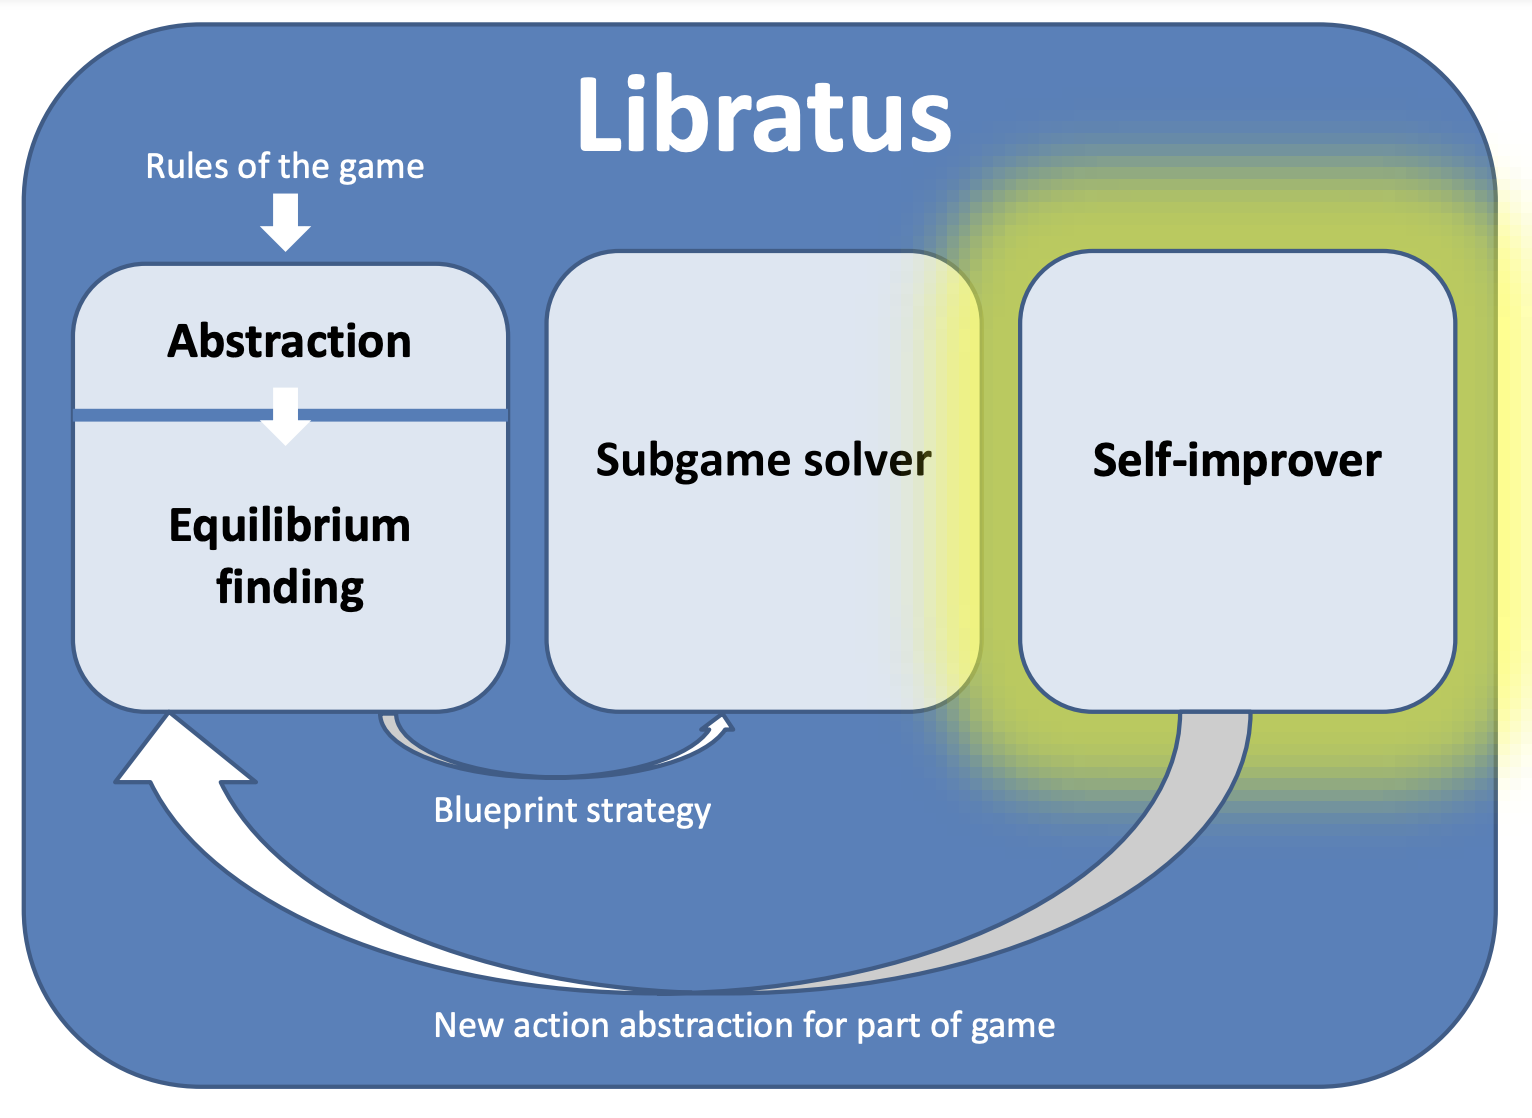
\includegraphics[width=6.26772in,height=4.56944in]{media/media/image5.png}

\textbf{\ul{HOW IT OVERCOMES THE IMPERFECT INFORMATION OBSTACLE:}}

\begin{quote}
Libratus effectively addresses the challenge of imperfect information by
employing a combination of abstraction, real-time subgame solving, and
self-improvement. The abstraction process reduces the complexity of the
game, allowing Libratus to focus on strategically significant decisions
without being overwhelmed by the vast number of possible game states. By
using nested subgame solving, Libratus can refine its strategy in real
time, adapting to the specific circumstances of each hand. This approach
ensures that Libratus can manage the uncertainty inherent in poker,
making informed decisions even when some information is hidden. The
self-improving algorithm further enhances Libratus\textquotesingle s
ability to adapt by learning from opponents\textquotesingle{} actions
and refining its strategy accordingly (Brown \& Sandholm, 2018).
\end{quote}

\textbf{\ul{RELATION TO MULTI-AGENT LEARNING:}}

\begin{quote}
Libratus is related to multi-agent learning primarily through its use of
self-play to refine its strategies. While it is not a multi-agent system
in the traditional sense of interacting with multiple autonomous agents
simultaneously, Libratus does simulate interactions with an opponent to
improve its strategy. This process involves learning from the actions
and potential strategies of a single opponent, which is a form of
multi-agent learning. By iteratively playing against itself, Libratus
can explore a wide range of scenarios and adapt its strategy to optimize
performance.
\end{quote}

\textbf{\ul{LIMITATIONS:}}

\begin{itemize}
\item
  Specific to two-player games
\item
  Computational Demands
\item
  Libratus does not explicitly exploit opponents' weaknesses. Instead,
  it focuses on maintaining a robust strategy that is difficult to
  exploit, which may limit its ability to capitalize on specific
  opponent tendencies.
\end{itemize}

\textbf{\ul{STRENGTHS:}}

\begin{itemize}
\item
  Does a diverse range of betting sizes, from small bets to large
  all-ins. It can make it difficult for opponents to predict Libratus's
  hand strength based solely on bet size (adds unpredictability).
\item
  In any given situation, Libratus can choose from multiple bet sizes.

  \begin{itemize}
  \item
    This can allow it to tailor its strategy to the specific context of
    the hand (therefore optimizing based on the current game state and
    other variables like opponent behavior).
  \end{itemize}
\item
  ``Limping'' (calling the big blind rather than raising), ``donk
  betting'' (betting into the previous round's aggressor). These strong
  tactics can catch opponents off guard and disrupt their expectations.
\item
  ``Perfect balance'' via maintaining equilibrium. Causes the agent to
  not be as easily exploitable.
\item
  A mixed strategy uses probability distributions over possible actions
  rather than committing to a single deterministic approach. This
  randomness is important because it makes it challenging for opponents
  to predict Libratus's next move.
\item
  Probability distribution over players' hands, not just
  ``range-based''.
\item
  Near-perfect subgame play; great use of ``blockers'' (cards that
  reduce the likelihood of opponents having certain hands)
\end{itemize}

\textbf{\ul{FUTURE WORK DIRECTIONS:}}

\textbf{\ul{PLURIBUS:}}

\textbf{\ul{SUMMARY:}}

\begin{quote}
Pluribus is an AI system developed by Noam Brown and Tuomas Sandholm, in
collaboration with Facebook AI Research, designed to play six-player
no-limit Texas Hold\textquotesingle em poker. It represents a
significant advancement in AI\textquotesingle s ability to handle
multiplayer imperfect-information games. In a series of experiments,
Pluribus consistently defeated elite human professionals (and by a large
margin), demonstrating its capability to navigate the complex
interactions of multiplayer poker (Brown \& Sandholm, 2019).
\end{quote}

\textbf{\ul{HOW IT WORKS (HIGH LEVEL):}}

\begin{quote}
Pluribus begins by running Monte Carlo Counterfactual Regret
Minimization (MCCFR) in self-play to produce an offline ``blueprint''
strategy for the entire six-player game. Unlike full CFR, MCCFR samples
a subset of actions at each decision point, dramatically reducing
computation while still driving regrets toward equilibrium. To keep the
blueprint tractable, Pluribus also applies action and information
abstraction, grouping similar bet sizes and merging analogous game
states.

Once play begins against human or AI opponents, Pluribus uses its
precomputed blueprint as a safe, high-level plan but then refines it in
real time. Whenever the current hand reaches a decision point, Pluribus
conducts a shallow, focused search over that subgame, again using
abstraction, to adjust its strategy to the specific situation. This
two-phase approach (offline blueprint + online subgame search) balances
scalability with responsiveness.

Because multiplayer Nash equilibria can be prohibitively expensive to
compute, and may not even yield the best practical performance, Pluribus
does not target an exact equilibrium. Instead, it relies on its
blueprint for overall safety and its localized real-time solutions to
exploit opportunities as they arise. Crucially, however, Pluribus does
not continuously learn or track opponent tendencies during a match; its
robustness comes from the combination of a sound blueprint and
judicious, on-the-fly subgame refinement rather than from
opponent-specific adaptation.
\end{quote}

\textbf{\ul{HOW IT OVERCOMES THE IMPERFECT INFORMATION OBSTACLE:}}

Pluribus is designed to work in multi-agent environments (multiplayer
poker). It must navigate interactions with multiple players, each with
their own strategies and objectives. This setting inherently involves
multi-agent dynamics, as Pluribus must consider the potential actions
and strategies of several opponents simultaneously. It refines its
strategies through self-play, where it plays against copies of itself.
This process allows Pluribus to explore a wide range of scenarios and
develop strategies that are robust in a multiplayer context. By
simulating interactions with multiple agents, Pluribus effectively
engages in a form of multi-agent learning during its training phase.
Also accomplishes this due to robust pre-computed strategies.

\textbf{\ul{RELATION TO MULTI-AGENT LEARNING:}}

\begin{quote}
Pluribus exemplifies multi-agent learning by navigating interactions
with multiple players, each with their own strategies and objectives.
This requires the AI to adapt and learn from the actions of several
agents simultaneously, demonstrating the potential of AI to learn and
adapt in dynamic, competitive environments. Pluribus also plays against
other iterations of itself, which can be considered multi-agent learning
as well.
\end{quote}

\textbf{\ul{LIMITATIONS:}}

\begin{quote}
While Pluribus demonstrates strong empirical performance (beating Poker
professionals decisively), achieving equilibrium in multiplayer games is
more challenging, and its strategies are not guaranteed to be optimal in
all scenarios (even if equilibrium is found).. Importantly, Pluribus
plays a fixed strategy and does not adapt to the observed tendencies of
opponents during live play. This design choice focuses on maintaining a
robust overall strategy rather than exploiting specific opponent
weaknesses.

\textbf{\ul{COST TO USE:}}

The blueprint strategy for Pluribus was computed in 8 days on a 64-core
server for a total of 12,400 CPU core hours. It required less than 512
GB of memory. At current cloud computing spot instance rates, this would
cost about \$144 to produce.

This is in sharp contrast to all the other recent superhuman AI
milestones for games, which used large numbers of servers and/or farms
of graphics processing units (GPUs).

More memory and computation would enable a finer-grained blueprint that
would lead to better performance but would also result in Pluribus using
more memory or being slower during real-time search.

set the size of the blueprint strategy abstraction to allow Pluribus to
run during live play on a machine with no more than 128 GB of memory
while storing a compressed form of the blueprint strategy in memory.
\end{quote}

\textbf{\ul{STRENGTHS:}}

\begin{itemize}
\item
  It is extremely computationally efficient. It achieves this incredible
  performance with relatively modest computational resources compared to
  other AI systems like AlphaGo.
\item
  Pluribus maintains a strong, consistent strategy that is difficult for
  human opponents to exploit.
\item
  Through real-time search and abstraction, Pluribus can adapt its
  strategy to the specific context of each game situation, though it
  does not adapt based on opponent behavior (which could be a strength).
\end{itemize}

\begin{quote}
\textbf{\ul{FUTURE WORK DIRECTIONS:}}
\end{quote}

\begin{itemize}
\item
  Developing methods to exploit specific opponent tendencies while
  maintaining a robust overall strategy could enhance
  Pluribus\textquotesingle s performance. If a more offensive profile
  was developed (aka adapting based on opponent behavior), Pluribus
  could be even better. This is worth exploring.
\end{itemize}

\textbf{\ul{CONCLUSION}}

Over the last two decades, AI has progressed from brute-force search in
perfect-information games (DeepBlue) to deep learning plus tree search
(AlphaGo) and, most recently, to rigorously grounded, game-theoretic
approaches for hidden-information environments (Libratus and Pluribus).
At the heart of these breakthroughs is the realization that:

\begin{enumerate}
\def\labelenumi{\arabic{enumi}.}
\item
  Abstraction dramatically reduces complexity. Grouping similar bet
  sizes or hand patterns lets CFR-based algorithms solve otherwise
  intractable poker variants.
\item
  Blueprint + subgame Solving provides a safe, high-level plan online
  while allowing real-time refinement in the critical decision points
  you actually reach.
\item
  Live Adaptation (via opponent modeling or repeated subgame solves) is
  essential to exploit human tendencies and guard against non-stationary
  bluff patterns---pure equilibrium play alone isn't enough.
\end{enumerate}

\textbf{\ul{REFERENCES:}}

\begin{itemize}
\item
  Brown, N., \& Sandholm, T. (2018). Superhuman AI for heads-up no-limit
  poker: Libratus overcomes human talent. Science, 359(6374), 418--424.
  \href{https://doi.org/10.1126/science.aao1733}{\ul{https://doi.org/10.1126/science.aao1733}}
\item
  Brown, N., \& Sandholm, T. (2019). Pluribus: The first AI to beat pros
  in multiplayer no-limit Texas hold 'em poker. Science, 365(6456),
  885--890.
  \href{https://doi.org/10.1126/science.aay2400}{\ul{https://doi.org/10.1126/science.aay2400}}
\item
  Campbell, M., Hoane, A. J., Jr., \& Hsu, F. H. (2002). Deep Blue.
  Artificial Intelligence, 134(1--2), 57--83.
  \href{https://doi.org/10.1016/S0004-3702(01)00129-1}{\ul{https://doi.org/10.1016/S0004-3702(01)00129-1}}
\item
  Silver, D., Huang, A., Maddison, C. J., Guez, A., Sifre, L., Van Den
  Driessche, G., ... \& Hassabis, D. (2016). Mastering the game of Go
  with deep neural networks and tree search. Nature, 529, 484--489.
  \href{https://doi.org/10.1038/nature16961}{\ul{https://doi.org/10.1038/nature16961}}
\item
  Kuhn, H. W. (1950). A simplified two-person poker. In H. W. Kuhn \& A.
  W. Tucker (Eds.), Contributions to the theory of games (Vol. I, pp.
  97--103). Princeton University Press.
\item
  More DeepBlue:

  \begin{itemize}
  \item
    \href{https://www.sciencedirect.com/science/article/pii/S0004370201001291}{\ul{https://www.sciencedirect.com/science/article/pii/S0004370201001291}}
  \end{itemize}
\item
  Google AlphaGo:

  \begin{itemize}
  \item
    \href{https://www.nature.com/articles/nature16961}{\ul{https://www.nature.com/articles/nature16961}}
  \end{itemize}
\item
  Nash:

  \begin{itemize}
  \item
    \href{https://search.lib.utexas.edu/discovery/openurl?institution=01UTAU_INST&vid=01UTAU_INST:SEARCH&rft.aulast=Nash&rft.volume=54&url_ver=Z39.88-2004&rft_id=info:doi\%2F10.2307\%2F1969529&rft.date=1951&rft.spage=286&rft.jtitle=Ann.\%20Math.&rft.aufirst=J.&rft.atitle=Non-Cooperative\%20Games&rft.title=Ann.\%20Math}{\ul{https://search.lib.utexas.edu/discovery/openurl?institution=01UTAU\_INST\&vid=01UTAU\_INST:SEARCH\&rft.aulast=Nash\&rft.volume=54\&url\_ver=Z39.88-2004\&rft\_id=info:doi\%2F10.2307\%2F1969529\&rft.date=1951\&rft.spage=286\&rft.jtitle=Ann.\%20Math.\&rft.aufirst=J.\&rft.atitle=Non-Cooperative\%20Games\&rft.title=Ann.\%20Math}}.
  \item
    \href{https://www.jstor.org/stable/1969529?origin=crossref&seq=1}{\ul{https://www.jstor.org/stable/1969529?origin=crossref\&seq=1}}
  \end{itemize}
\item
  Neumann:

  \begin{itemize}
  \item
    \href{https://link.springer.com/article/10.1007/BF01448847}{\ul{https://link.springer.com/article/10.1007/BF01448847}}
  \item
    Helpful video:
    \href{https://www.youtube.com/watch?v=NrJpVhuieK4&ab_channel=AbdelazizBahnasy}{\ul{https://www.youtube.com/watch?v=NrJpVhuieK4\&ab\_channel=AbdelazizBahnasy}}
  \end{itemize}
\item
  Libratus video explanation

  \begin{itemize}
  \item
    \href{https://www.youtube.com/watch?v=2dX0lwaQRX0}{\ul{https://www.youtube.com/watch?v=2dX0lwaQRX0}}
  \end{itemize}
\item
  \href{https://en.wikipedia.org/wiki/Lee_Sedol}{\ul{https://en.wikipedia.org/wiki/Lee\_Sedol}}
\item
  \href{http://modelai.gettysburg.edu/2013/cfr/cfr.pdf}{\ul{http://modelai.gettysburg.edu/2013/cfr/cfr.pdf}}
\end{itemize}

\end{document}
